% 
\documentclass[11pt]{article}

% Polskie znaki
%-------------------------------------
% \usepackage{polski}
\usepackage[english]{babel}
\usepackage[utf8]{inputenc}
\usepackage[T1]{fontenc}
% Page settings
%------------------------------------
\usepackage{geometry}
\geometry{
	a4paper,
	%total={170mm,257mm},
	left=15mm,
	right=15mm,
	top=15mm,
	bottom=15mm,
}
% justify
\setlength\parindent{10pt}
% no paragraph indent
\usepackage{ragged2e}
% Header
%--------------------------
\usepackage{fancyhdr}
\usepackage{wrapfig}
\pagestyle{fancy}
\fancyhf{}
\rhead{Summer Semester 2023/24}
\lhead{1000-719bMSB}
\rfoot{\thepage}

% hyperlinks
\usepackage{hyperref}
\usepackage{lipsum}
% Report title
%------------------------------------------

\title{\vspace{-15mm}
    {\textbf{\centering {Exploration and re-analysis of a cellular subpopulation study using scRNA-seq data from melanoma samples}\\
			\vspace{5mm}
			\large \emph{Modeling of Complex Biological Systems}
   \vspace{-5mm}
}}}
\author{\textit{Younginn Park}}

% Abstract
\date{\begin{adjustwidth}{30pt}{30pt}
		\vspace{2mm}
		{\normalsize Melanoma is a highly malignant form of skin cancer that continues to pose significant challenges due to its complex cellular heterogeneity and metastatic potential. This project aims to re-examine the computational methods for single-cell transcriptomics applied to data from 19 melanoma patients in the 2016 study by Tirosh et al\cite{tirosh_dissecting_2016}. Findings from this project emphasize the importance of dimensionality reduction techniques for effective visualization and grouping of cells by their transcriptional profiles, while revealing some of the limitations of trajectory analysis. Inter-cellular heterogeneity, which was explored separately for malignant and non-malignant cells, was observed among cells in both subsets and improved upon the original study by applying feature selection steps. Malignant cells displayed heterogeneity by clustering around each of the distinct patient's tumor samples, which suggests uniqueness of each cancer's transcriptional profiles. On the other hand, non-malignant cells clustered around cell types demonstrating distinctness of transcriptomes of those cell types with some exceptions. However, the analysis of intra-cellular heterogeneity in selected malignant cells was less straightforward, falling short of revealing clear subpopulations, complicating the immediate application of trajectory inference.
  }
        \vspace{2mm}
\end{adjustwidth}}

% Space between sections
%--------------------------------------------
\usepackage[compact]{titlesec}
\titlespacing{\section}{0pt}{2ex}{2ex}
\titlespacing{\subsection}{0pt}{1ex}{1ex}
\titlespacing{\subsubsection}{0pt}{0.5ex}{0ex}


% Multi column sections
%-------------------------------------
\usepackage{multicol}

% Colors in latex tables
\usepackage[table,xcdraw]{xcolor}
\usepackage{multirow}
% Figure captions
\usepackage{caption}
\usepackage{subcaption}

% Math symbols
%-----------------------------------
\usepackage{mathtools}

% Tags for equations
%------------------------------------
\newcommand\addtag{\refstepcounter{equation}\tag{\theequation}}

% Importing images
%--------------------------------
\usepackage{graphicx}
\graphicspath{ {./plots/} } % define folder for images
% \graphicspath{ {../plots/} } % alternative

% Custom margins for texts
\usepackage{changepage}

\renewcommand{\familydefault}{\rmdefault}


\usepackage[sectionbib, super, comma, sort&compress]{natbib}

\usepackage{etoolbox}
\patchcmd{\thebibliography}{\chapter*}{\section*}{}{}



\begin{document}

\maketitle

\thispagestyle{fancy}

\vspace{-10mm}

\section{Introduction}
\vspace{-4mm}
\begin{multicols}{2}
    \noindent
    Melanoma is responsible for the majority of skin cancer-related deaths worldwide\cite{heistein_malignant_2024}. Melanoma cells are known for their ability to rapidly proliferate and metastasize, posing significant challenges for effective treatment. According to recent statistics, the incidence of melanoma has been steadily increasing, making it a critical focus of cancer research\cite{noauthor_melanoma_2015}. Understanding the molecular and cellular mechanisms underlying melanoma progression is essential for developing more targeted and effective therapies.

    The tumor microenvironment in melanoma is highly complex, comprising not only malignant cells but also a variety of immune cells. These immune cells, which include, but are not limited to T cells, B cells, macrophages, and natural killer cells, play crucial roles in the tumor's behavior and response to treatment\cite{tirosh_dissecting_2016}. Their gene expression profiles can provide valuable insights into the interactions between the tumor and the immune system, influencing both tumor growth and the efficacy of immunotherapies.

    This project's exploration and re-evaluation will be based on a 2016 study by a team of researchers from Broad Institute of MIT and Harvard\cite{tirosh_dissecting_2016}, which explored the transcriptional landscape of melanomas based on 19 selected patients that were in different stages of medication, age, sex and type of identified oncogenic mutation linked to the development of the tumor. The goal of this re-analysis will be to test alternative computational approaches from those used in the original study, aiming to improve the results obtained in them. 
    
    This re-analysis study will focus on two aspects of analyzing single cell transcriptomic data that involves dimension reduction - cluster analysis, which focuses on inter-cellular heterogeneity, which helps identify cellular subpopulations, and trajectory analysis, which can help illustrate intra-cellular heterogeneity that results from temporal processes that a certain cell subpopulation might be undergoing, in this case the focus will lie on malignant melanoma cells.

\end{multicols}
    
\subsection{Transcriptional characteristics of melanoma tissues}
\begin{multicols}{2}
    \noindent
    Single-cell RNA sequencing (scRNA-seq) has emerged as a powerful tool for dissecting the cellular heterogeneity within tumors\cite{chen_single-cell_2023}. This technology allows researchers to go beyond aggregate analyses of transcripts in order to reveal gene expression at the individual cell level, uncovering distinct cellular subpopulations and their unique transcriptional profiles. By applying scRNA-seq to melanoma samples, it is possible to gain a deeper understanding of the tumor's cellular composition and the molecular pathways driving its progression.
    
    In the context of melanoma, the transcriptome can reveal critical information about the disease. Melanoma cells exhibit diverse transcriptional characteristics, with specific genes and pathways being differentially expressed. For instance, the study under re-analysis identified that all tumors harbored malignant cells from two distinct transcriptional cell states. Tumors characterized by high levels of the MITF transcription factor also contained cells with low MITF and elevated levels of the AXL kinase. These two transcriptional profiles, MITF and AXL, have significant implications for prognosis and treatment response\cite{muller_low_2014}.
    
    MITF is a key regulator in melanoma, crucial for the development, differentiation, and survival of melanocytes. High MITF levels are typically associated with a high proliferation, low metastasis of cancer phenotype. Conversely, AXL is linked to the invasive and metastatic behavior of melanoma, making it an attractive target for cancer therapies\cite{simmons_brn2_2022}. The inverse correlation between MITF and AXL expression suggests a complex regulatory network influencing melanoma cell behavior, with high MITF levels corresponding to low AXL expression and vice versa.

\end{multicols}
    
\subsection{Overview of computational methods}
\begin{multicols}{2}
    \noindent
    Dimensionality reduction is a critical step in the analysis of single-cell RNA sequencing data, helping in both feature selection and visualization. In the context of scRNA-seq, where thousands of genes are measured across thousands of cells, not all genes contribute equally to the variability observed among the cells. Dimensionality reduction techniques help to simplify this complex data by reducing the number of dimensions, i.e. genes, while presenting the most significant sources of variability. This reduction is essential for uncovering the underlying structure of the data, making it more interpretable and manageable for downstream analyses, such as clustering and trajectory inference. Most notable methods for dimension reduction that will be used in this project include Principal Component Analysis (PCA), t-distributed Stochastic Neighbor Embedding (t-SNE) and Uniform Manifold Approximation (UMAP).

    \subsubsection{Dimensionality reduction}
    \noindent
    PCA is a linear dimensionality reduction technique that transforms high-dimensional data into a new coordinate system\cite{pearson_liii_1901}. Each principal component is a linear combination of the original genes, with the first capturing the highest variance and subsequent components capturing decreasing amounts of variance. PCA is simple, fast, and interpretable, making it useful for initial data exploration and visualization. However, it assumes linear relationships between genes, which may not capture complex, nonlinear structures in the data. For this reason, two other methods are also taken into consideration.

    Both t-SNE and UMAP are non-linear dimensionality reduction methods commonly used in scRNA-seq data analysis. t-SNE excels at preserving local structure by modeling each high-dimensional object as a two- or three-dimensional point, ensuring that similar objects are represented by nearby points and dissimilar objects by points that are distant with high probability. This feature is particularly effective for visualizing complex datasets and accurately identifying clusters\cite{maaten_visualizing_2008}. However, it is computationally intensive, and can struggle with large datasets, making the results less interpretable. UMAP, on the other hand, models the data as uniformly distributed on a Riemannian manifold with a locally constant (or approximated) metric, and ensuring the manifold is locally connected. It can often provides more meaningful representations of the overall data structure\cite{mcinnes_umap_2018}. Despite these advantages, UMAP’s low-dimensional representations can still be challenging to interpret directly in terms of the original high-dimensional gene expression data. Moreover, both t-SNE and UMAP are stochastic methods, which can sometimes pose a challenge when it comes to reproducibility. To summarize, all methods are invaluable for visualizing scRNA-seq data, but they come with trade-offs regarding computational demands, visual clarity and interpretability.

    \subsubsection{Clustering}

    Clustering in single-cell RNA sequencing (scRNA-seq) data analysis is essential for identifying distinct cellular subpopulations based on gene expression profiles. Two of the popular clustering methods are DBSCAN (Density-Based Spatial Clustering of Applications with Noise) and Shared Nearest Neighbors (SNN). DBSCAN is advantageous for its ability to detect arbitrarily shaped clusters in a more intuitive way by first grouping cells that are closer together with many neighbors and identify outliers as noise without requiring a predefined number of clusters\cite{ester_density-based_1996}. This makes it particularly useful for heterogeneous scRNA-seq data where the number of cell types is unknown. However, DBSCAN's performance is sensitive to the choice of parameters such as the neighborhood radius (epsilon) and the minimum number of neighboring points, which can be challenging to set optimally for complex scRNA-seq datasets.

    Shared Nearest Neighbors (SNN) clustering is another method for clustering cells in a scRNA-seq dataset\cite{kumari_et_al_scalable_2016}. In this method, first a k-nearest neighbors (KNN) graph is constructed, which is then used to build the SNN graph by computing the neighborhood overlap (Jaccard index) between each cell and its k nearest neighbors. SNN does not require the number of clusters to be predefined, allowing for the dynamic detection of diverse cell populations. Other popular clustering algorithms include k-Nearest Neighbors and k-means.

    \subsubsection{Trajectory analysis}

    The other kind of analysis that can be performed on transcriptional data is trajectory analysis. In the study of living tissues, datasets of gene expression levels offer a sort of snapshots of dynamic processes unfolding across cells. This approach allows for a unique approach for an analysis that aims to order these expression levels along a continuum of expression profiles ordering them in a unit referred to as pseudotime\cite{trapnell_dynamics_2014}. Pseudotime reflects different stages of temporal processes within cells, rather than actual time, and captures transitions between different cell identities. This analytical perspective seeks to identify paths that minimize expression level differences between cells, recreating a developmental timeline. By mapping changing gene expression across pseudotime can provide insights into biological processes and temporal progression. Tools like Monocle\cite{trapnell_dynamics_2014} and Wanderlust\cite{bendall_single-cell_2014} are valuable for conducting trajectory inference within computational environments.
    
\end{multicols}


% Methods
\section{Methods}

\subsection{Data collection and pre-processing}
\begin{multicols}{2}
    \noindent
    The data from single cell RNA-seq from the original study was made available through the GEO database (Gene Expression Omnibus)\cite{barrett_ncbi_2013} under accession code GSE72056\cite{noauthor_geo_nodate}. Tissue biopsy collection method was described in the Supplementary Material 1 of the original study. Single cell isolation was conducted using FACS (Fluorescence-activated Cell Sorting), which consisted of creating suspensions of cells, staining and separating them using specific antibodies for cell types and calcein for fluorescent marking all per kits' manufacturers' recommendations (VWR, Life Technologies and BioLegend), while excluding doublets using forward (FSC) and sideward (SSC) scatter in the flow cytometry apparatus. Amplification was done using a modified SMART-Seq2 protocol with Maxima Reverse Transcriptase (Life Technologies). The products of previous step were then cleaned and Illumina sequencing libraries were prepared using Nextera XT (Illumina), assessed (Agilent) and quantified (Life Technologies). Sequencing was done using Illumina NextSeq 500 in 30 bp paired-end mode.

    In order to normalize transcript read count, sequenced paired-end reads were mapped to USCS hg19 human transcriptome using Bowtie with specific parameters that allows alignment of sequences that differ by a point mutation. The read count data for gene $i$ and sample $j$ was then normalized using TPM with the following formula:

    $$E_{i,j} = log_2 (\frac{TPM_{i,j}}{10 + 1})$$

    Here TPM was divided by 10 because of the assumption of the researchers for the libraries to be of complexity in the order of 100,000 and would avoid inflating the difference between cells with genes detected and no genes detected. When the data was pooled for certain populations of cells for an aggregated metric, the division by 10 was omitted and the expression level was then calculated using:

    $$E_p(I)=log_2(TPM(I)+1)$$

    Further filtering of cells was then conducted by removing cells with fewer than 1,700 genes detected or when the average expression of manually curated list of housekeeping genes (Table S16 in the Supplementary Material 1 of Tirosh et al.\cite{tirosh_dissecting_2016}) following the above formula for $E_p$ was less than 3. Further filtering of remaining cells by aggregate expression below 4 was done. The final step was to calculate the relative expression levels for the remaining cells and genes by centering them using the following formula:

    $$Er_{i,j}=E_{i,j} - average[E_{i,1...n}]$$

    The resulting expression matrix from the GEO database consisted of 4,645 cells with 23,686 features. 3,256 cells were classified as non-malignant, 1,257 as malignant and 132 remained unresolved. The matrix from the database contained no information about technical variables, but had metadata with tumor ID that is synonymous with patient's biopsy ID, information about the cell's malignancy status and for the non-malignant cells - information about the type of immune cell that the cell has been classified to. This expression matrix from GEO database was first imported into Seurat. Mitochondrial genes were being searched for, but none were found, so it's assumed that they were also removed by the researchers. The distribution of the number of features and feature counts was explored (Figure \ref{fig:pre-process}). Since there are no significant outliers and since some preliminary filtering was already done by the original researchers there will be no further filtering in this project in order to be as permissive as possible.
    
\end{multicols}

\begin{figure}
    % \centering
    \begin{subfigure}{.5\textwidth}
      \centering
      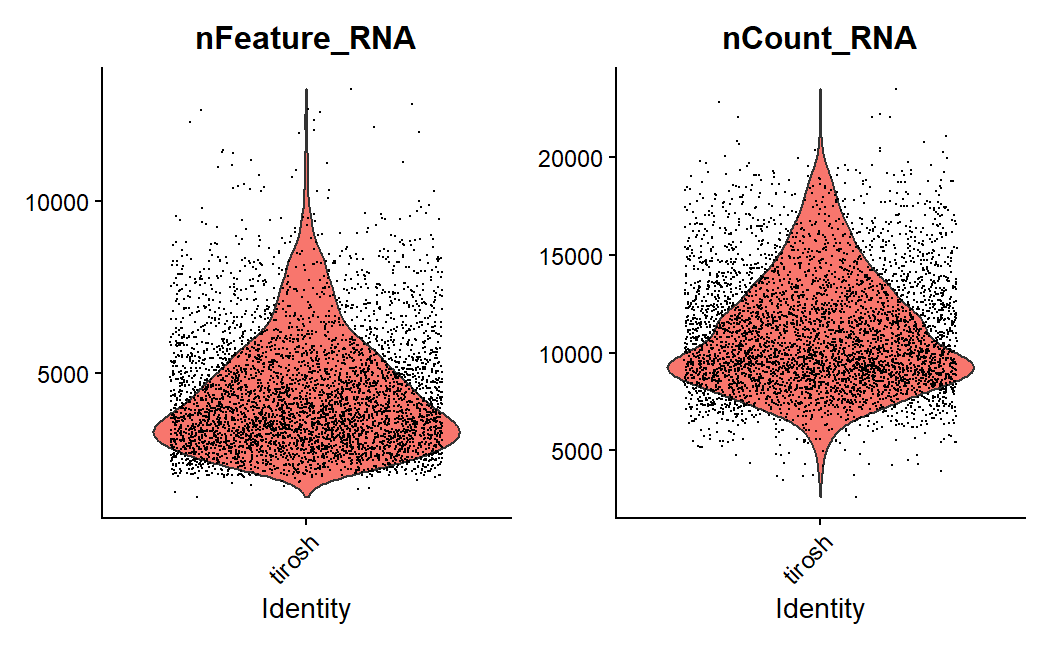
\includegraphics[width=.9\linewidth]{plots/plot_md-vln.png}
      \caption{}
      \label{fig:vln}
    \end{subfigure}
    \begin{subfigure}{.5\textwidth}
      \centering
      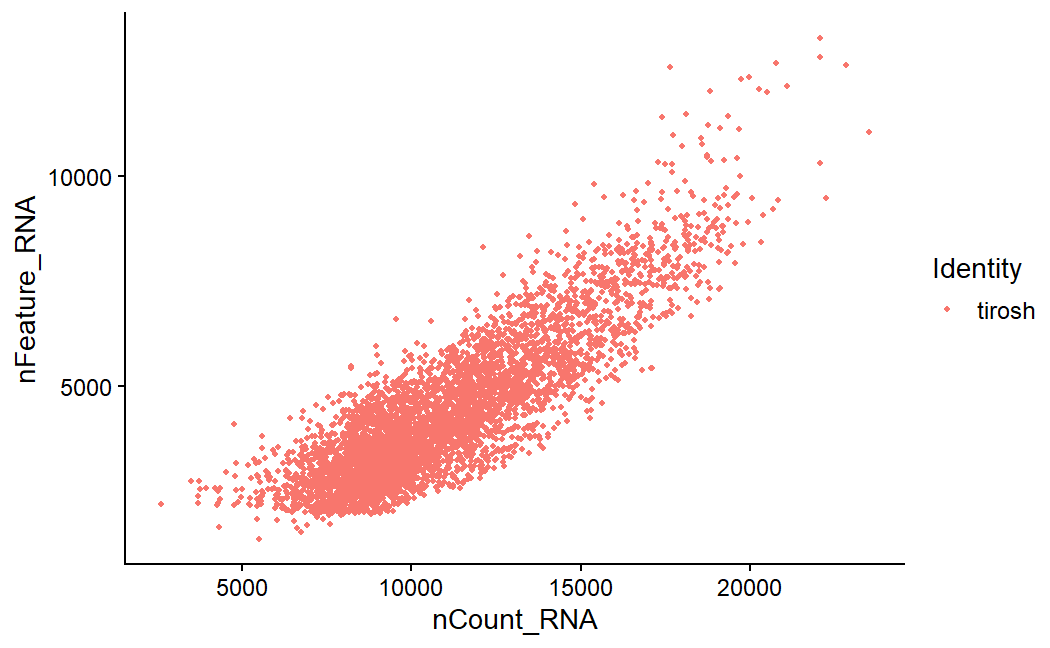
\includegraphics[width=.9\linewidth]{plots/plot_md-scat.png}
      \caption{}
      \label{fig:scat}
    \end{subfigure}
    \caption{Results from quality control of the scRNA-seq dataset from the original study: a) Violin plots of number of features and feature counts across cells; b) Scatter plot of number of features against feature counts.}
    \label{fig:pre-process}
\end{figure}

\subsection{Dimensionality reduction and cluster analysis}
\begin{multicols}{2}
    \noindent
    In the original study, t-SNE was utilized for marker identification and visualization of cellular subpopulations (Matlab implementation with dim=15). However, the original analysis imposed on itself a major limitation - due to the increased complexity of t-SNE visualization with a higher number of tumors, the analysis was limited to 13 tumors with at least 100 cells each, and further restricted to 6 tumors samples with more than 50 malignant cells for the malignant cell subset. The original study also doesn't mention any feature variability analysis.

    Thus this project will attempt to improve this approach by utilizing all tumor samples, applying a feature selection method and doing visualization using t-SNE and UMAP (\textit{n.components}=2, \textit{n.neighbors}=10). Variance Stabilizing Transformation (VST) from Seurat (seurat reference) will be used to select 1,000 most variable features. This approach is promising in mitigating the effects of noise and redundant signals from transcriptional data and reduce the computational complexity by selecting the most informative genes, by variability in this case.
    
    In the original study, to define cell types from the non-malignant t-SNE analysis, a density clustering method, DBscan, was employed. This approach revealed six clusters which were subsequently characterized by the top preferentially expressed genes, which included multiple known markers of specific cell types. Consequently, the researchers identified clusters corresponding to T cells, B cells, macrophages, endothelial cells, cancer-associated fibroblasts (CAFs), and NK cells. This method relied on prior knowledge of marker genes that help indentify major cell types.

    A slightly modified version of kNN from Seurat v5 [hao 2024], called SNN will be used (\textit{resolution}=0.1) as an alternative method for DBSCAN. All of these will be done using R programming language. Different parameters will be tested in order to obtain roughly the same number of clusters as in the original study.
    
\end{multicols}


\subsection{Trajectory analysis}
\begin{multicols}{2}
    
    \noindent
    The original study identified intra-cellular heterogeneity based on two distinct transcriptional programs - MITF and AXL. Both of these programs of malignant cells were identified through principal component analysis (PCA), with components PC2-6 being associated with various biological processes: cell cycle (PC2 and 6), regional heterogeneity (PC3), and the MITF expression program (PC4 and 5). Then the top 100 genes most correlated with MITF across all malignant cells were selected to define the MITF program, and their average relative expression was calculated as the MITF-program cell score. Conversely, the average expression of the top 100 genes that negatively correlated with the MITF program scores defined the AXL program and were used to compute the AXL-program cell score (Figure \ref{fig:tirosh-mitf}).

    The original study's use of PCA to identify the MITF and AXL programs in malignant cells effectively highlighted key biological processes and provided a structured approach to quantify gene expression variability. However, while PCA efficiently captures linear correlations and simplifies complex data, it may overlook non-linear relationships and finer intra-cellular heterogeneity that involves different expression programs. Additionally, focusing solely on the top 100 correlated genes might miss other significant contributors to cellular behavior. Incorporating trajectory analysis could address these limitations by capturing dynamic changes and developmental pathways within the cells, offering a more comprehensive understanding of cellular heterogeneity and progression.

    To improve upon the original analysis and trying to make it more systematic for similar studies, a trajectory analysis will be attempted using Monocle v3 in R programming language\cite{trapnell_dynamics_2014}. Different dimension reduction methods will be examined including t-SNE, UMAP and Latent Semantic Indexing (LSI), implemented in Monocle. Tumor sample \textit{Mel79} was selected for this analysis for its highest representation in the dataset.

    \begin{center}
        \captionsetup{type=figure}
        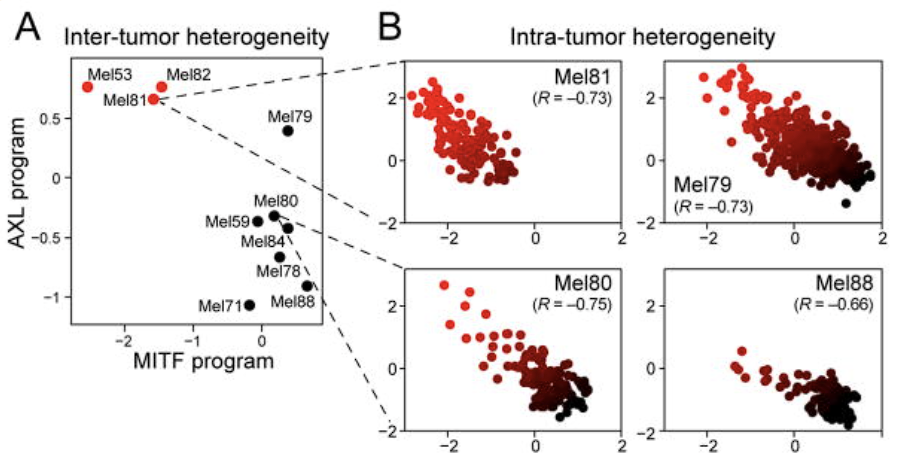
\includegraphics[width=8cm]{plots/tirosh_mitf_axl.png}
        \caption{The results of the original analysis of the MITF and AXL expression program that involved creating custom components (MITF-AXL program scores) based on expression levels of relevant marker genes (fragment of Figure 3. from Tirosh et al. 2016}
        \label{fig:tirosh-mitf}
    \end{center}

\end{multicols}


\section{Results}

\subsection{Cluster analysis}

\begin{center}
    \captionsetup{type=figure}
    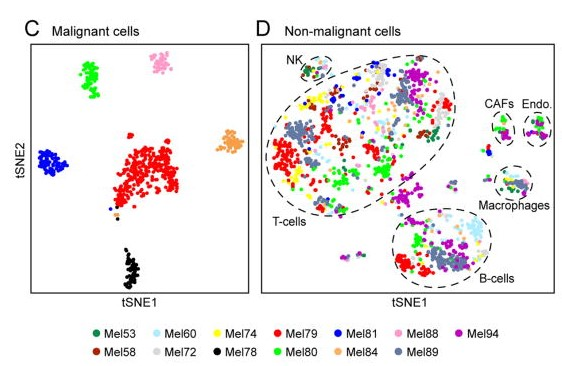
\includegraphics[width=15cm]{plots/tirosh_plots.jpg}
    \caption{Clustering results from the original study obtained through t-SNE with dims=15, colored by tumor ID (fragment of Figure 1. from Tirosh et al. 2016). Left: Clustering of malignant cells for selected 6 tumor samples. Right: Clustering of non-malignant cells for selected 13 tumor samples.}
    \label{fig:tirosh_plots}
\end{center}


\begin{figure}
    % \centering
    \begin{subfigure}{.5\textwidth}
      \centering
      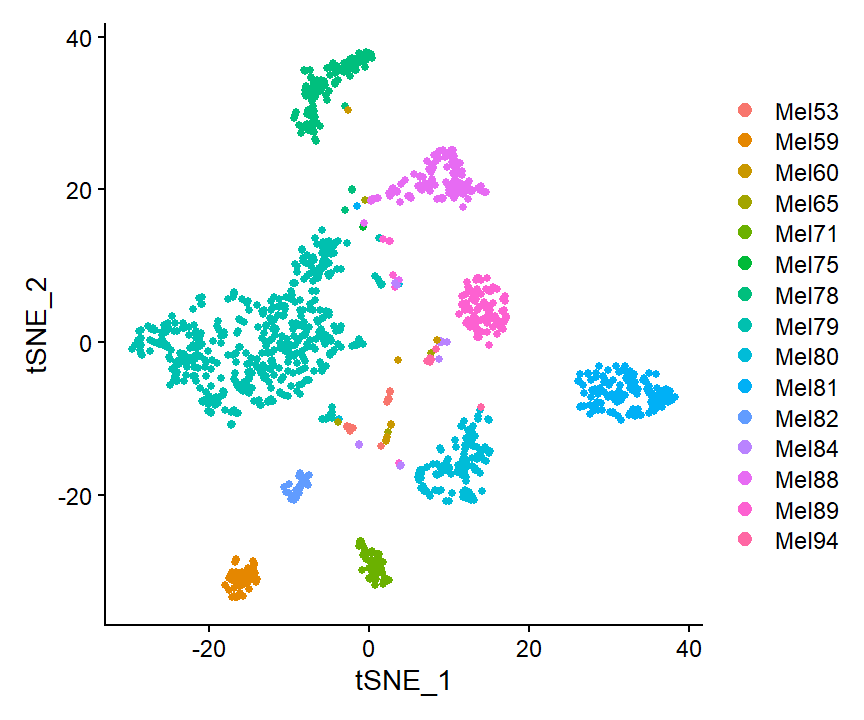
\includegraphics[width=.9\linewidth]{plots/plot_m-tsne-novf-tumor.png}
      \caption{}
      \label{fig:m-tsne-novf}
    \end{subfigure}
    \begin{subfigure}{.5\textwidth}
      \centering
      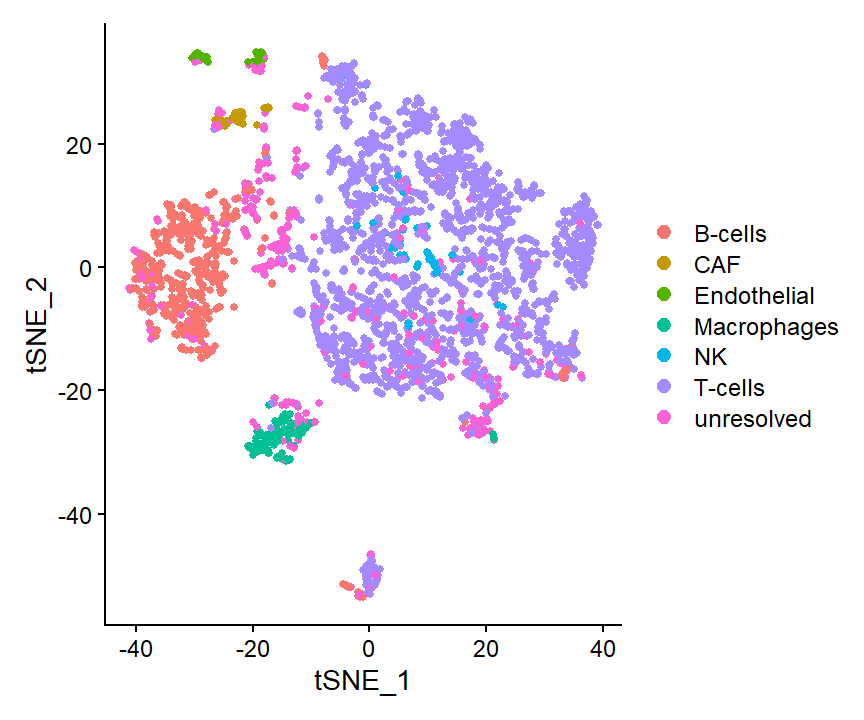
\includegraphics[width=.9\linewidth]{plots/plot_nm-tsne-novf-cell.png}
      \caption{}
      \label{fig:nm-tsne-novf}
    \end{subfigure}
    \begin{subfigure}{.5\textwidth}
      \centering
      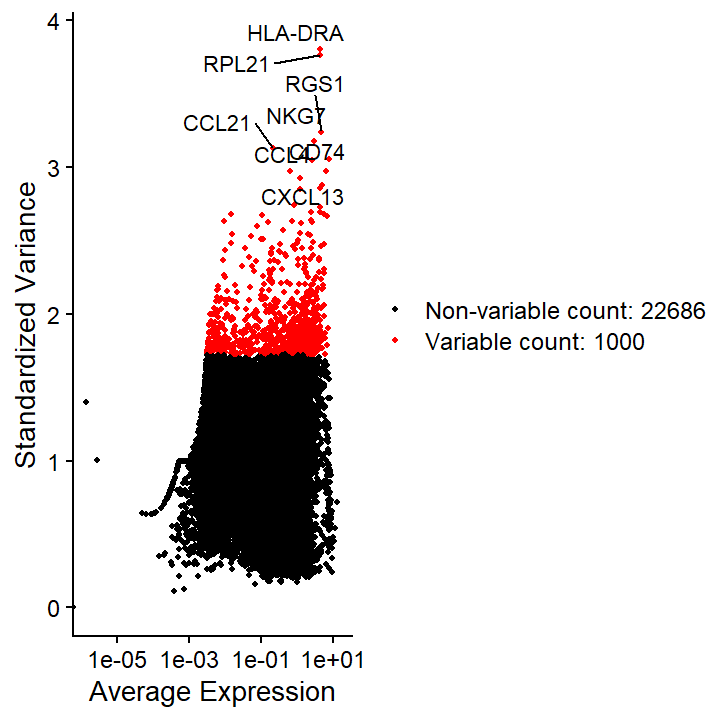
\includegraphics[width=.9\linewidth]{plots/plot_vf-top10.png}
      \caption{}
      \label{fig:vf-top10}
    \end{subfigure}
    \begin{subfigure}{.5\textwidth}
      \centering
      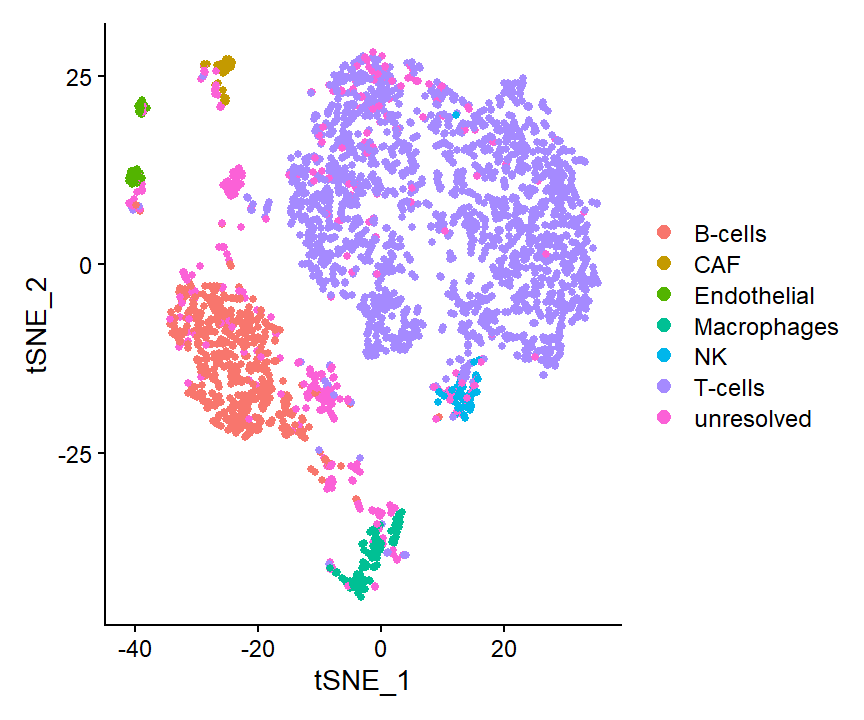
\includegraphics[width=.9\linewidth]{plots/plot_nm-tsne-vf-cell.png}
      \caption{}
      \label{fig:nm-tsne-vf}
    \end{subfigure}
    \caption{Various visualizations from the analysis: a) Reconstruction of malignant cells t-SNE using dim=15 with all genes for dimension reduction, clusters colored by tumor ID; b) Reconstruction of non-malignant cells t-SNE using dim=15 with all genes for dimension reduction, clusters colored by cell type; c) Variable feature plot with top 1000 variable genes colored in red and top 10 variable genes labeled by name; d) t-SNE visualization of non-malignant cells using dim=15 based on variable features, clusters colored by cell type.}
    \label{fig:dim-red-figures}
\end{figure}


\begin{multicols}{2}

    \subsubsection{Dimension reduction}
    \noindent
    First, reproductions of the original study were conducted, separately for malignant and non-malignant cells. For malignant cells, t-SNE visualization with dim=15 revealed clear heterogeneity among tumors. Although the results were not perfectly identical to those of the original study, similar distinct clusters for most tumor samples were observed, except for a few samples that had limited representation in the original dataset (Figure \ref{fig:m-tsne-novf}).

    For non-malignant cells, t-SNE clustering also mirrored the findings of the original study (Figure \ref{fig:nm-tsne-novf}). However, several challenges were encountered. Notably, NK cells appeared within the cluster originally assigned to T-cells in this visualization. Additionally, a small portion of T-cells formed a separate cluster apart from the main grouping. Endothelial cells also formed two distinct groups, a pattern that did not emerge in the original study.

\end{multicols}


    % \begin{center}
    %     \captionsetup{type=figure}
    %     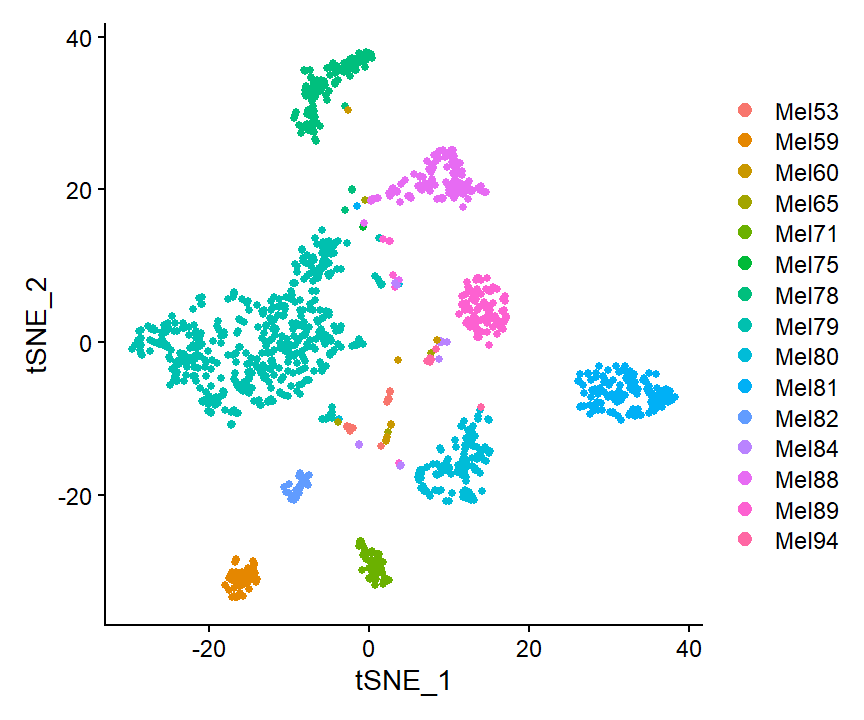
\includegraphics[width=8cm]{plots/plot_m-tsne-novf-tumor.png}
    %     \caption{Reconstruction of malignant cells t-SNE using dim=15 using all genes for dimension reduction, clusters colored by tumor ID}
    %     \label{fig:m-tsne-novf}
    % \end{center}

    % \begin{center}
    %     \captionsetup{type=figure}
    %     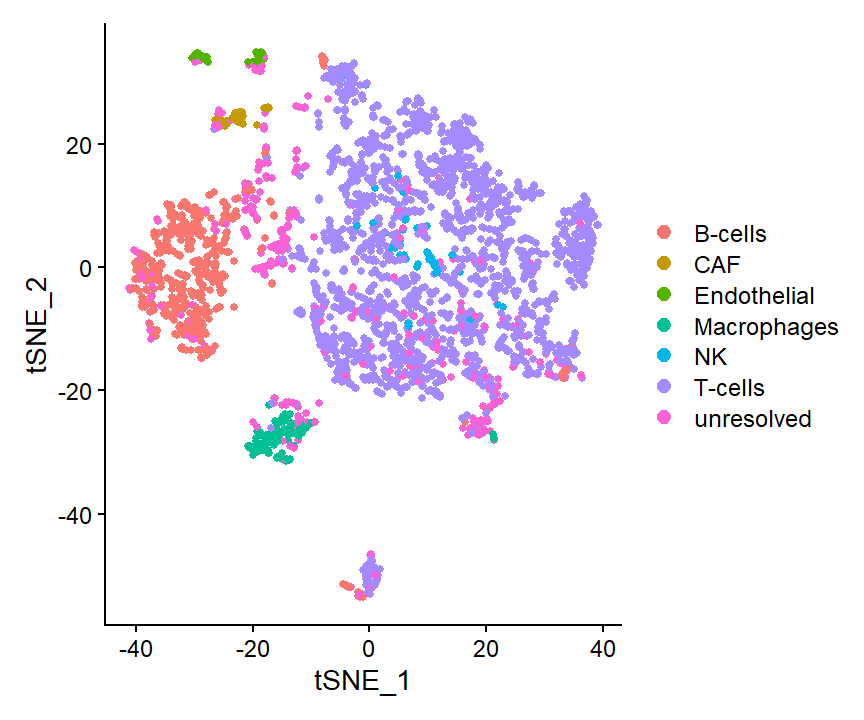
\includegraphics[width=8cm]{plots/plot_nm-tsne-novf-cell.png}
    %     \caption{Reconstruction of non-malignant cells t-SNE using dim=15 using all genes for dimension reduction, clusters colored by cell type}
    %     \label{fig:nm-tsne-novf}
    % \end{center}

    % \begin{center}
    %     \captionsetup{type=figure}
    %     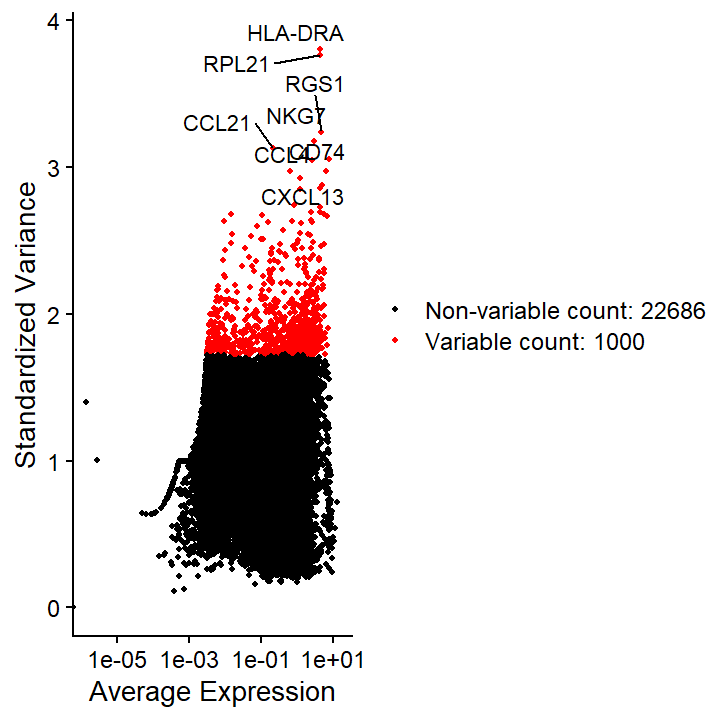
\includegraphics[width=8cm]{plots/plot_vf-top10.png}
    %     \caption{Variable feature plot with top 1000 variable genes colored in red and top 10 variable genes labeled by their name}
    %     \label{fig:vf-top10}
    % \end{center}

    % \begin{center}
    %     \captionsetup{type=figure}
    %     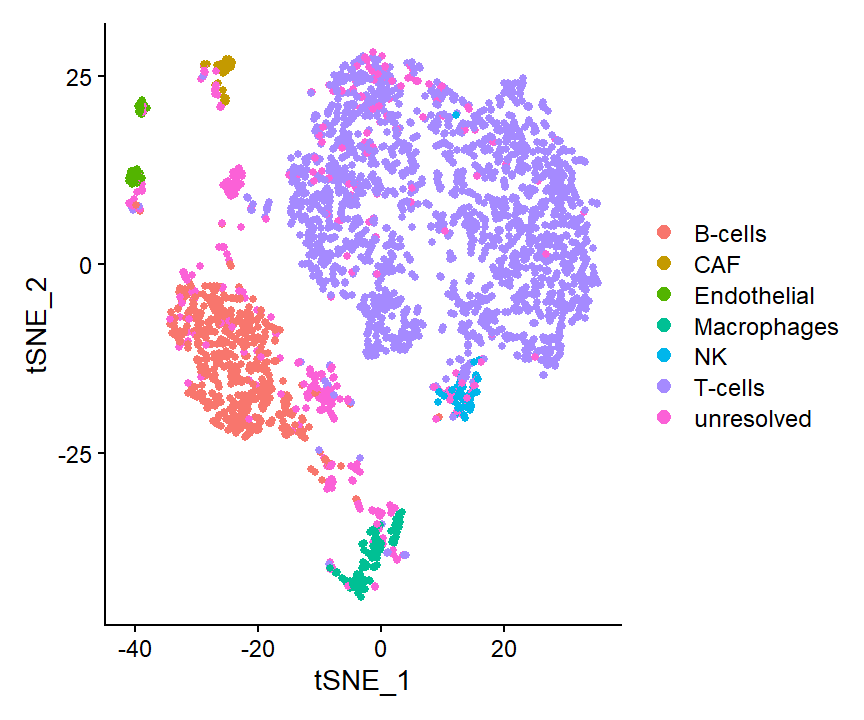
\includegraphics[width=8cm]{plots/plot_nm-tsne-vf-cell.png}
    %     \caption{t-SNE visualization of non-malignant cells on dim=15 based on variable features, clusters colored by cell type}
    %     \label{fig:nm-tsne-vf}
    % \end{center}

\begin{multicols}{2}

    \subsubsection{Variable features analysis}
    \noindent
    To improve the results of dimension reduction visualization, the 1000 most variable features were used for further analysis (Figure \ref{fig:vf-top10}). Both t-SNE (Figure \ref{fig:nm-tsne-vf} and UMAP (Figure \ref{fig:nm-umap-vf}) were utilized at this stage.

    Variable feature analysis with VST appeared to aid with NK cells, which now formed a visually separate cluster. T-cells also seem to form a more uniform cluster, although two emerging subpopulations can be observed, which is more clearly visible in UMAP (Figure \ref{fig:nm-umap-vf}). Both t-SNE and UMAP visualizations were unable to merge the endothelial cells, resulting in two separate clusters of roughly the same size.

    \begin{center}
        \captionsetup{type=figure}
        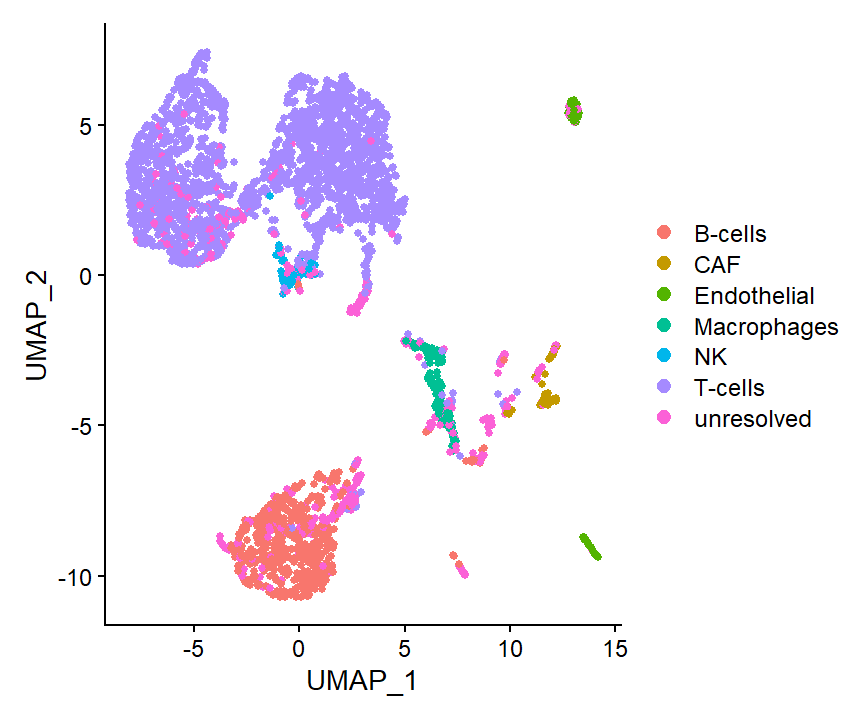
\includegraphics[width=8cm]{plots/plot_nm-umap-vf-cell.png}
        \caption{UMAP visualization of non-malignant cells on dim=15 based on variable features, clusters colored by cell type}
        \label{fig:nm-umap-vf}
    \end{center}

    The clear separation of malignant tumor cells into distinct clusters raised a question regarding batch effects. Since tumor ID refers to the separate patient biopsy samples, it is the only available technical variable in the dataset. Basic checks of PCs against each other, t-SNE, and UMAP colored by tumor ID revealed no major clustering around this variable, which suggests that batch effects were already accounted for by the original researchers and were not present in this dataset.


    \subsubsection{Cluster inference}
    \noindent
    After the analysis of the PCs formed from variable features, 15 PCs were used to conduct clustering with the SNN algorithm. UMAP was employed to visualize the resulting clusters as it appeared to form the most distinct and separate clusters, aiding in the analysis of the inferred 7 clusters (Figure \ref{fig:nm-umap-vf-snn}). This clustering revealed heterogeneity in T-cells, identifying two subpopulations of T-cells, integrating NK cells into one of those subpopulations and separating endothelial cells into two distinc clusters.

    \begin{center}
        \captionsetup{type=figure}
        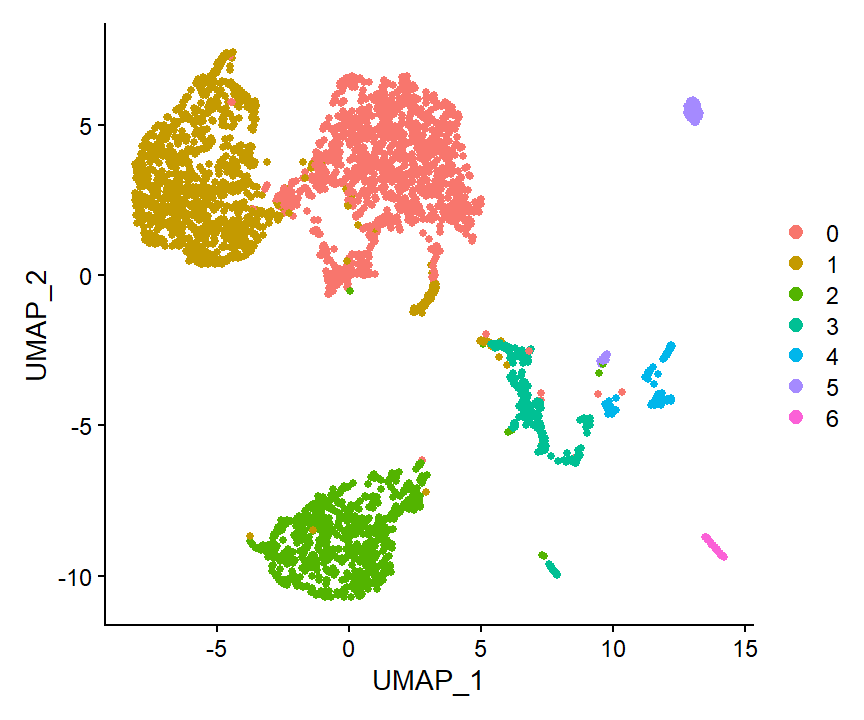
\includegraphics[width=8cm]{plots/plot_nm-umap-vf-snn.png}
        \caption{UMAP visualization of non-malignant cells on dim=15 based on variable features, clusters colored by groups obtained using SNN clustering}
        \label{fig:nm-umap-vf-snn}
    \end{center}

\end{multicols}


\subsection{Trajectory analysis}
\begin{multicols}{2}
    \noindent
    Trajectory analysis was conducted on malignant cells from sample \textit{Mel79}. Among various dimensionality reduction techniques, UMAP provided the most visually informative results (Figure \ref{fig:t-umap}). When cells were colored based on MITF and AXL expression (Figure \ref{fig:t-umap-mitf}), no distinct heterogeneity or subpopulations were revealed. Further analysis involved constructing learned graphs and trajectories to identify potential clusters representing different cell states or stages of a biological process (Figure \ref{fig:t-umap-order}).

    \begin{center}
        \captionsetup{type=figure}
        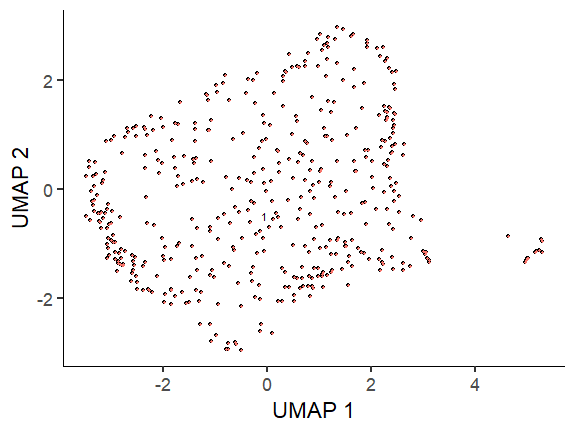
\includegraphics[width=4cm]{plots/plot_t-umap.png}
        \caption{UMAP visualization of cells in tumor sample \textit{Mel79}}
        \label{fig:t-umap}
    \end{center}

    However, the results were unsatisfactory as the expected distinct clusters did not emerge. Monocle ultimately recognized only a single cluster, failing to provide insights into the diverse cellular states or transitions within the malignant cells. This outcome suggests that additional methods or refinements may be necessary to uncover meaningful heterogeneity and dynamic processes in this dataset.

    \begin{center}
        \captionsetup{type=figure}
        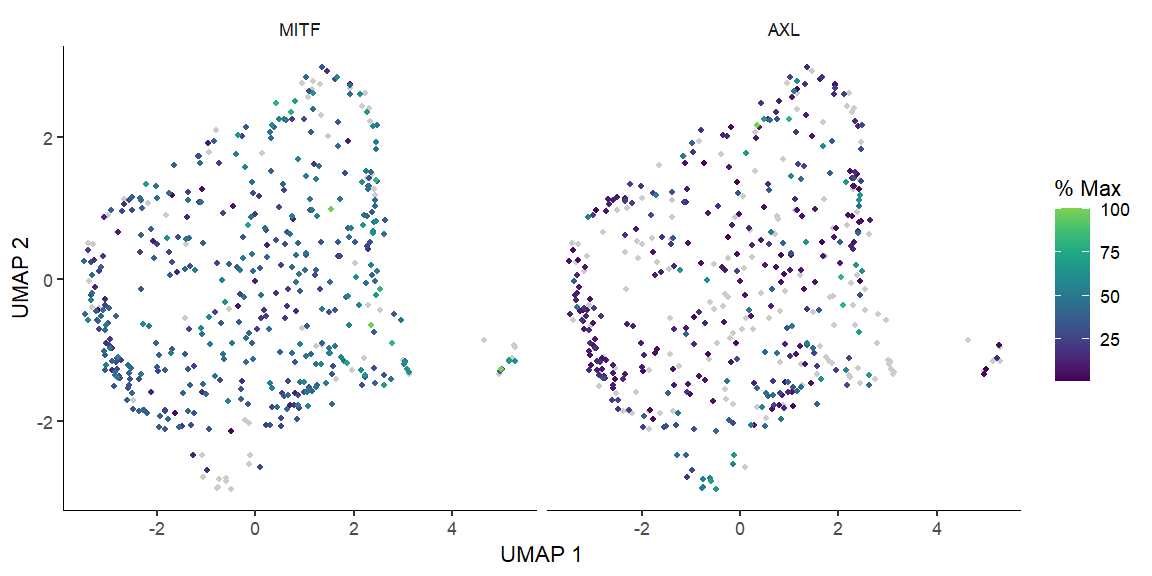
\includegraphics[width=8cm]{plots/plot_t-umap-mitf-axl.png}
        \caption{UMAP visualization of tumor sample \textit{Mel79} with cells marked with expression levels for MITF (left) and AXL (right)}
        \label{fig:t-umap-mitf}
    \end{center}

    Analogous analyses were done on malignant cells from tumor \textit{Mel78} and \textit{Mel88}, but similarly without visible success in finding intra-cellular heterogeneity from the above method.
    
    \begin{center}
        \captionsetup{type=figure}
        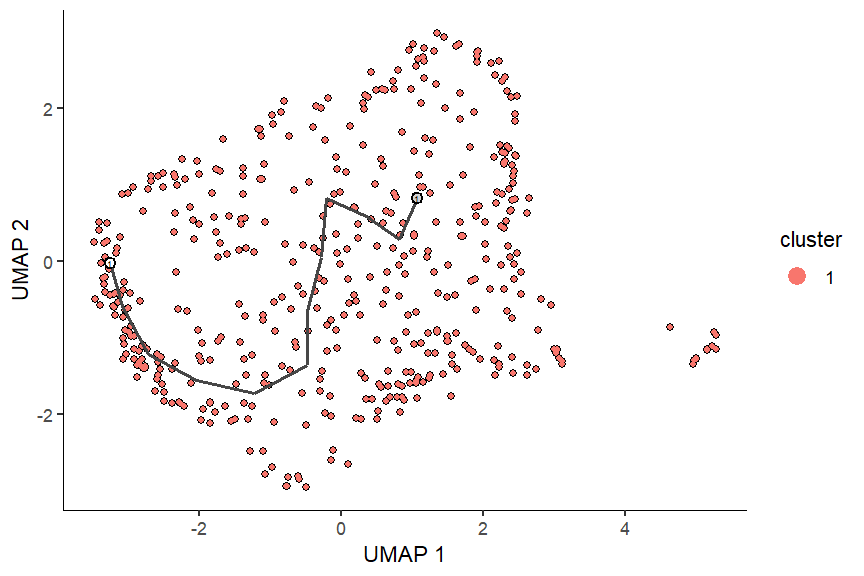
\includegraphics[width=8cm]{plots/plot_t-umap-order.png}
        \caption{UMAP visualization of tumor sample \textit{Mel79} with a graph attempting to show the ordering of cells in pseudotime.}
        \label{fig:t-umap-order}
    \end{center}

\end{multicols}

      
\section{Discussion}
    \begin{multicols}{2}
    \noindent
    Starting with dimension reduction methods, it is essential to evaluate which method yielded the best visualization. Both t-SNE and UMAP, following feature selection, produced the most visually informative results. Among these, UMAP showed a clearer separation of clusters, which could be fine-tuned using the $n.neighbors$ parameter to adjust the level of granularity.
    
    One of the challenges encountered was the difficulty in exactly replicating the dimension reduction methods such as t-SNE and UMAP, owing to their inherently stochastic nature. This randomness can lead to variability in the results across different runs, making direct comparisons or replications challenging.
    
    An important consideration was the uniqueness of all tumor samples. The saying "no two cancers are the same" holds true here, but also raised the question of whether the observed variability was due to biological uniqueness or batch effects. The original study did not mention adjusting for any technical variables, leaving some uncertainty. However, since non-malignant cells did not cluster by tumor samples, it can be safely assumed that there were no significant technical variables that obscured relevant transcriptional data.

    For cluster inference, several key observations were made. Two distinct subpopulations of T-cells were identified, suggesting potential distinctions between various T-cell types such as regulatory T-cells (Tregs), cytotoxic T-cells (CD8+), or helper T-cells (Th). This finding indicates the complexity and functional diversity within the T-cell population in melanoma, which would require an additional analysis of marker genes.
    
    Additionally, significant heterogeneity was observed in endothelial cells, a phenomenon that has been reported in various studies of melanoma\cite{zeng_understanding_2023, maishi_tumor_2019}. This heterogeneity underscores the varied roles and states of endothelial cells within the tumor microenvironment, which may have implications for tumor progression, metastasis and treatment response\cite{maishi_tumor_2019}.
    
    Exploring alternative and potentially more advanced methods of feature (gene) selection, such as Jackstraw\cite{chung_statistical_2020} and Singular Value Decomposition (SVD\cite{klema_singular_1980} analyses, might have yielded better visualization and clustering results. These methods offer robust statistical frameworks for identifying significant features, potentially providing a more accurate representation of the underlying biological processes and improving the separation of cellular subpopulations in dimension reduction tasks.
    
    The results obtained from the SNN analysis differed considerably from those of the DBSCAN method used in the original study. This discrepancy highlights the need for further investigation to understand the underlying reasons for these differences. Factors such as parameter selection, sensitivity to noise, and the inherent characteristics of each clustering algorithm might contribute to the varied outcomes.

    The trajectory analysis did not proceed as smoothly as planned, raising questions about its effectiveness in capturing the expected cellular transitions in an ad hoc manner like in this project. Comparisons with references or studies that employed similar methodologies, but achieved better results could provide valuable insights into potential improvements\cite{liu_single_2024} by involving marker genes and feature selection.
    
    Traditional dimension reduction methods, such as those used in this study, failed to reveal the intra-cellular heterogeneity previously identified using manual marker gene selection and correlation-scoring methods in the original study. This discrepancy suggests limitations in the ability of simple dimension reduction techniques to capture subtle biological variations within cell populations.
    
    One possible explanation for the challenges encountered in trajectory analysis could be the relatively low cell count in the analyzed tumor sample (\textit{Mel79}) compared to different studies\cite{he_single-cell_2021}. \textit{Mel79} was the sample with the highest malignant cell representation in the dataset and it comprised of approximately one-third of all malignant cells in the dataset (468 cells). The limited sample size may have hindered the ability to discern meaningful cellular transitions or states.
    
    To enhance trajectory inference, employing variable feature analysis, similar to the approach used in cluster analysis, could potentially mitigate noise and improve the identification of biologically relevant gene expression patterns. By focusing on a subset of genes that exhibit significant variability across cells, rather than using all genes as done in this study, trajectory analysis could yield more robust and interpretable results.
    
    Addressing these considerations and implementing further improvements in future studies could enhance the efficacy and reliability of trajectory analysis in unraveling complex cellular processes. These enhancements would be crucial for advancing the understanding of cellular dynamics and their implications in diseases like melanoma.
    
    \end{multicols}

\newpage
\bibliographystyle{IEEEtran}
\bibliography{MBS} % citekey format: author_keyword_year

\end{document}
